\documentclass[12pt,a4paper]{article} %(nie wiem kiedy) usunąłem tą linię i nie wiem czy tak było
%przykladowe pakiety
\usepackage[utf8]{inputenc}
\usepackage{polski}
\usepackage{graphicx}
\usepackage{amsmath} % w zasadzie tez mozna wywalic 
\usepackage{booktabs}
\usepackage{listings}
\usepackage{color}
\usepackage{geometry} 
\usepackage{hyperref}
\usepackage{subcaption}

\geometry{
	a4paper,
	left = 2.5cm,
	right = 2.5cm,
	top = 2cm,
	bottom = 2cm
}

\begin{document}

\begin{titlepage}

\newcommand{\HRule}{\rule{\linewidth}{0.5mm}}

\center
 
\textsc{\LARGE Politechnika Wrocławska}\\[1.5cm] 
\textsc{\Large Zastosowanie informatyki w gospodarce}\\[0.5cm]

\HRule \\[0.5cm]
{ \huge \bfseries Relacje pomiędzy bytami w tekstach literackich, drugi kamień milowy.}\\[0.2cm]
\HRule \\[1.6cm]
 
 
\begin{minipage}{0.4\textwidth}
\begin{flushleft} \large
\emph{Lider grupy:}\\
Przemysław \textsc{Wujek} 234983\\
\emph{Skład grupy:}\\
Paweł \textsc{Czarnecki} 234974\\
Łukasz \textsc{Łupicki} 257536\\
Dawid \textsc{Piechota} 235851\\
Bartosz \textsc{Rodziewicz} 226105\\
Wojciech \textsc{Wójcik} 235621\\
\end{flushleft}
\end{minipage}
~
\begin{minipage}{0.4\textwidth}
\begin{flushright} \large
\emph{Prowadzący:} \\
dr inż. Tomasz \textsc{Walkowiak} 
\end{flushright}
\end{minipage}\\[4cm]

\vfill
{\large 27 maj 2020}

\end{titlepage}
   
\newpage

\section{Wczytywanie tekstów z plików}
    Interfejs użytkownika umożliwia wczytywanie tekstu podanego przez użytkownika ręcznie, oraz poprzez wczytanie pliku.
    
    \subsection{Obsługiwane formaty}
        Program aktualnie wspiera wczytywanie tekstu z plików tekstowych (np. txt) oraz plików PDF. Ekstrakcja tekstu z pdf jest wykonywana przez bibliotekę \texttt{pdf.js}. Operacja ta jest wykonywalna lokalnie na komputerze użytkownika. Plik pdf musi zawierać tekst, czytanie tekstu z obrazów (OCR) nie jest wspierane.
    
    \subsection{Ręczna modyfikacja}
        Po wczytaniu tekstu jest on uzupełniany do pola, w którym użytkownik może zmienić jego treść, usunąć część tekstu lub całkowicie zrezygnować z wysłania. Możliwe jest również ręczne uzupełnienie tego pola z pominięciem wczytywania pliku.
        
        \begin{figure}[h!]
            \centering
            \fbox{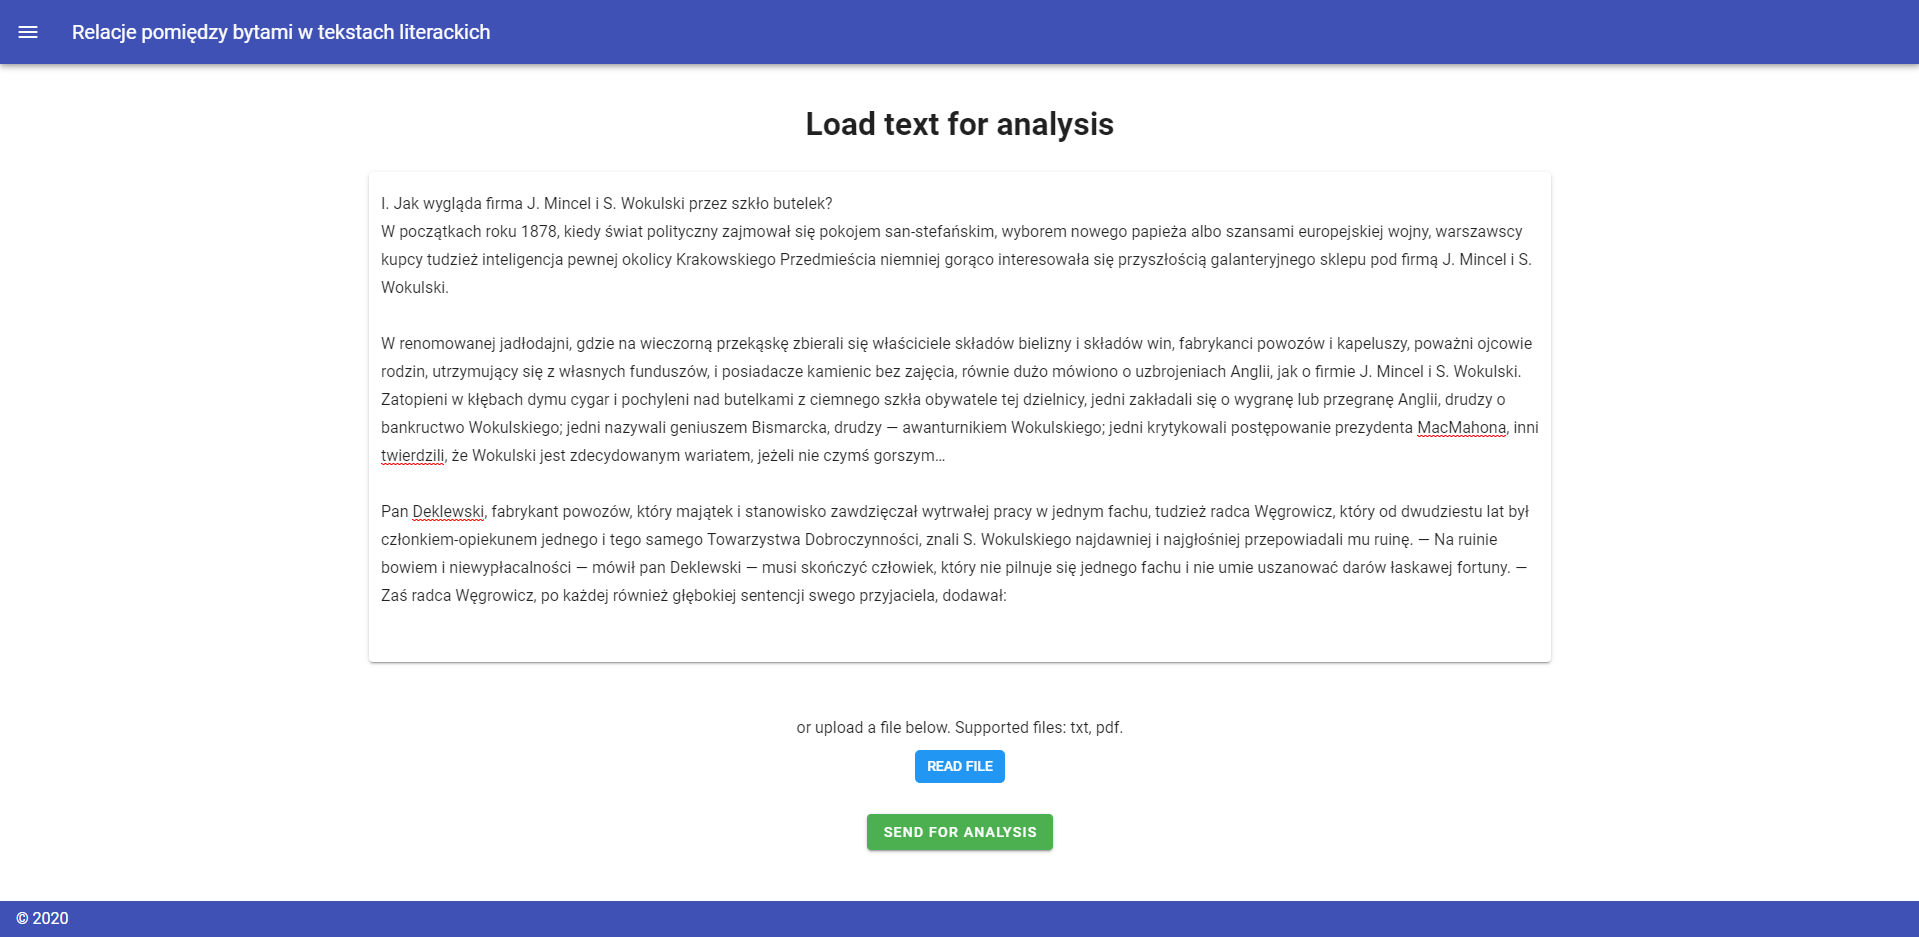
\includegraphics[width=0.9\textwidth]{rys/upload-tekstu.png}}
            \caption{Interfejs wczytywania tekstu}
        \end{figure}
        
    \subsection{Dane}
        Cały tekst książki pakowany jest w JSONa i wysyłany na RESTowy endpoint wystawiony przez backend.

\section{Dane dotyczące postaci z tekstu}

    \subsection{Dane}
        %jakie dane są zwracane
        %klasyfikacja połączeń i wystąpień postaci
        Dane zwracane z przeanalizowanego tekstu zwracają wagi połączeń pomiędzy bytami oraz liczbę wystąpień postaci na podstawie opisanej w wcześniejszym dokumencie metod wędrujących okien. Te dane wykorzystywane są w funkcji parsującej dane dla frontendu.\\
    
    \subsection{Format}
        %json, jakie wartości są zwracane
        Dane zwracane przez funkcje parsująca zawierają się w formacie danych JSON. Format prezentuje się następująco:
        \begin{lstlisting}
{
   "nodes": [
      {
         "name": "Pawel",
         "class": "rare"
      },
      {
         "name": "Przemek",
         "class": "rare"
      },
      {
         "name": "Wojtek",
         "class": "rare"
      },
      ...
   ],
   "links": [
      {
         "source": 0,
         "target": 1,
         "value": 244,
         "type": "straight"
      },
      {
         "source": 0,
         "target": 2,
         "value": 108,
         "type": "dotted"
      },
      {
         "source": 0,
         "target": 3,
         "value": 164,
         "type": "straight"
      },
      ...
   ]
}


        \end{lstlisting}
        
        Sekcja \textit{nodes} odpowiada za przekazanie danych wszystkich węzłów bytów wraz z ich nazwami(name) oraz sklasyfikowaną po stronie backendu częstością występowania(class). Częstość występowania zależna jest od maksymalnej wartości występowania postaci.\\
        
        Sekcja \textit{links} odpowiada za informacje dotyczące własności połączeń. Opisuje ona między którymi wierzchołkami następuje połączenie(source i target), wartość value, która określa moc połączenia(im większa tym silniejsze połączenie) oraz type, które określa jaki graficzny styl będzie miało połączenie wierzchołków. Styl \textit{straight} określa mocne połączenia, a styl \textit{dotted} słabe. Moc połączeń jest klasyfikowana odnosząc się do maksymalnej wartości połączenia.

\section{Zapis wyników do plików}

\subsection{Zapis modelu wykresu do pliku}

Do zapisania aktualnego stanu modelu do pliku wykorzystane zostało API przeglądarki do wygenerowania pliku, który następnie jest pobierany. Struktura pliku jest identyczna do tej opisanej w rozdziale 2.2. Przy wczytywaniu z pliku użytkownik wybiera plik z dysku z danymi wykresu.

\begin{figure}[!h]
    \center
        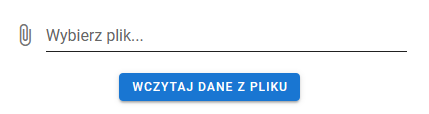
\includegraphics[scale=1]{rys/wojtek/1.png}
        \caption{Element UI odpowiadający za wczytanie danych grafu}
        \label{UIloadFile}
\end{figure}
W przypadku gdy ktoś niepoprawnie wypełni pole z wyborem pliku i kliknie przycisk {Wczytaj dane z pliku} zostanie mu wyświetlona informacja ukazana na rysunku \ref{uidialog}

\begin{figure}[!h]
    \center
        
\includegraphics[scale=1]{rys/wojtek/2.png}
        \caption{Komunikat informujący o braku pliku do wczytania}
        \label{uidialog}
\end{figure}
\subsection{Eksport wykresu do pliku graficznego}

Eksport wykresu odbywa się poprzez generowanie pliku PNG przez przeglądarkę. Jest on generowany na podstawie obecnej zawartości tagu \textit{<svg>} w którym znajduje się renderowany wykres. Plik graficzny zawiera legendę oraz wszystko co jest widoczne na wykresie w czasie kliknięcia przycisku \textit{Zapisz graf do pliku graficznego}. Takie działanie umożliwia ustawienie grafu w odpowiadającym użytkownikowi stanie i eksport tego grafu, jego części lub zbliżenia na daną część do pliku graficznego.

    %rodzaje plików, w jaki sposób dane są potem wczytywane z pliku, struktura pliku
\section{Prezentacja danych}
    %pokazanie screenów z metod prezentacji
    % podświetlenie
    % scalanie nodów
    % przemieszczanie nodów, tu opisać lekkie ograniczenie przez siły między nodami(później to będzie wyłączane?)
    
    
    \subsection{Coś o całości apliacji maybe}
    
    %sam nie wiem co tu napisać ale fajnie by było jakby był screen całej apki
    
    \begin{figure}[h!]
     \centering
      \fbox{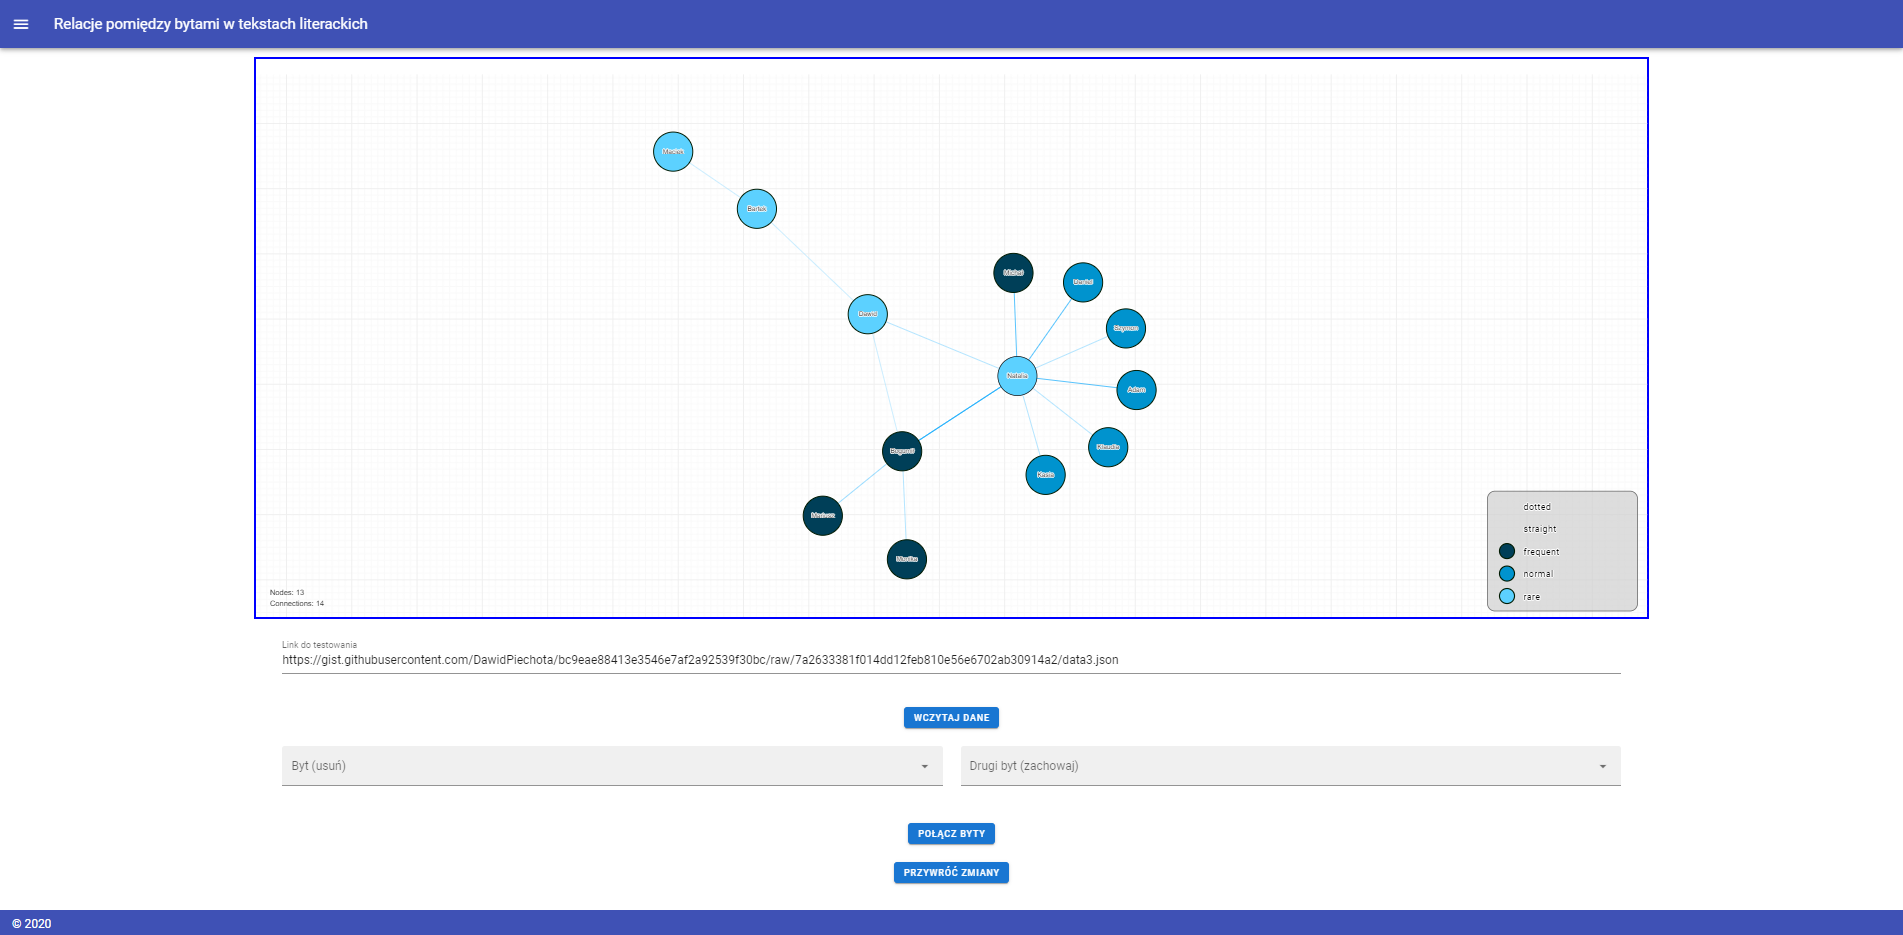
\includegraphics[width=0.9\textwidth]{rys/cala_apka.png}}
     \caption{front}
     \label{apka}
     \end{figure}
     
    \subsection{Łączenie mylnie rozdzielonych bytów}
    Użytkownik posiada możliwość ręcznego złączenia dwóch bytów w jeden [rys~\ref{fig:input}]. Funkcjonalność ta jest przydatna w przypadku gdy \textit{jak to się nazywało?} mylnie rozróżni jeden byt jako dwa osobne. Łączenie bytów polega na usunięciu pierwszego z nich oraz przypisaniu odpowiednich połączeń do bytu drugiego. Wynik takiej operacji został przedstawiony na rysunku \ref{fig:merge}. Wszelkie zmiany dokonane przez użytkownika mogą zostać przywrócone przyciskiem \textit{Przywróć zmiany}.
    
    \begin{figure}[h!]
    \centering
    \begin{subfigure}{.45\textwidth}
      \centering
      \fbox{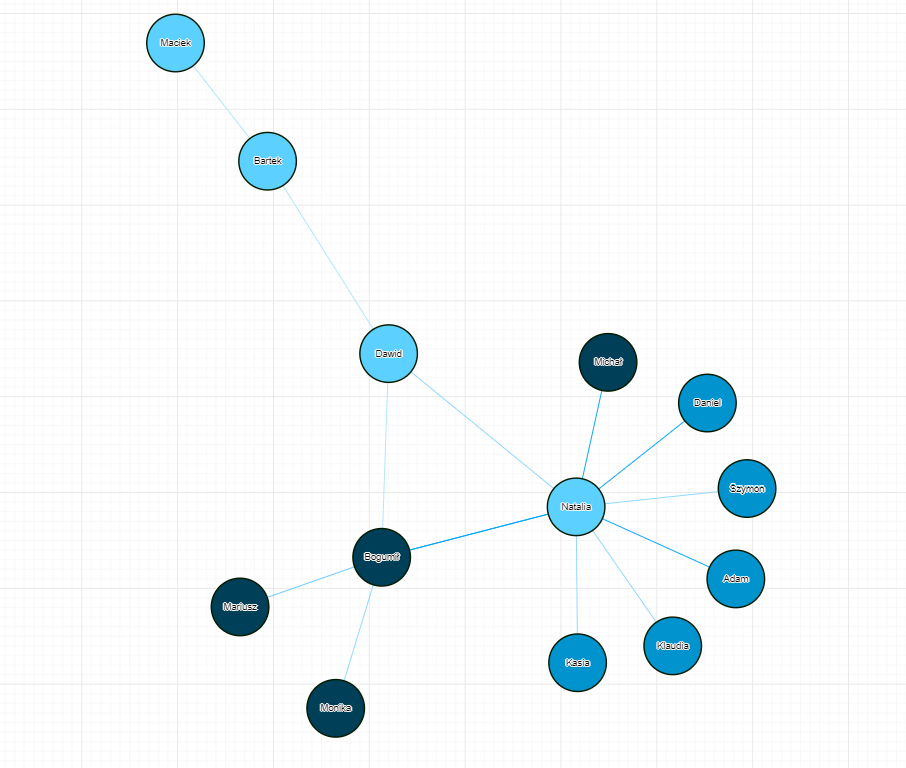
\includegraphics[width=.9\linewidth]{rys/merge_before.png}}
      \caption{Przed złączeniem}
    \end{subfigure}
    \begin{subfigure}{.45\textwidth}
      \centering
      \fbox{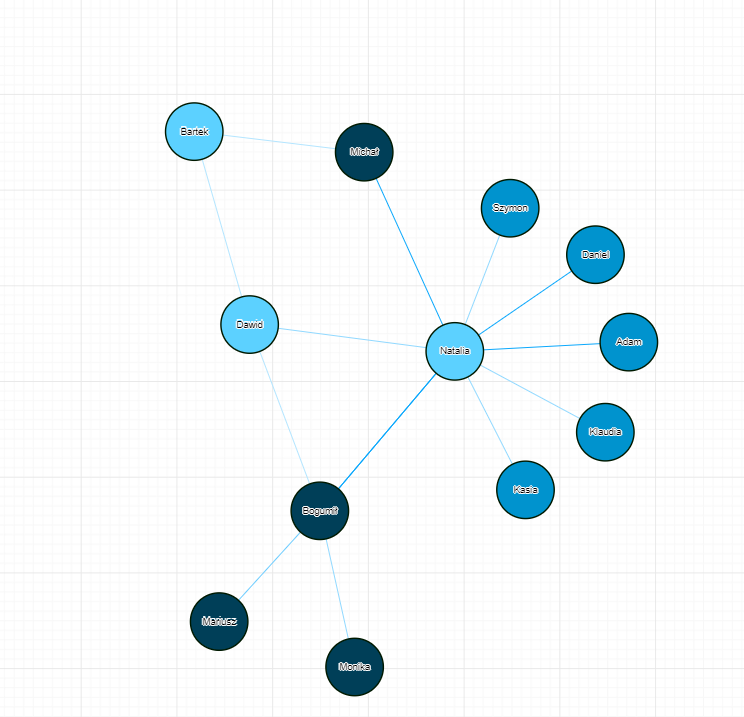
\includegraphics[width=.9\linewidth]{rys/merge_after.png}}
      \caption{Po złączeniu}
    \end{subfigure}
    \caption{Efekt złączenia bytów}
    \label{fig:merge}
    \end{figure}

    
    \begin{figure}[h!]
    \centering
    \begin{subfigure}{.45\textwidth}
      \centering
      \fbox{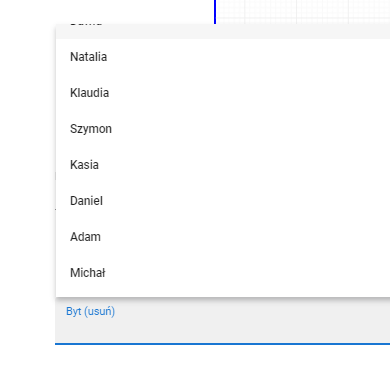
\includegraphics[width=.9\linewidth]{rys/nodes_list.png}}
      \caption{Lista}
    \end{subfigure}
    \begin{subfigure}{.45\textwidth}
      \centering
      \fbox{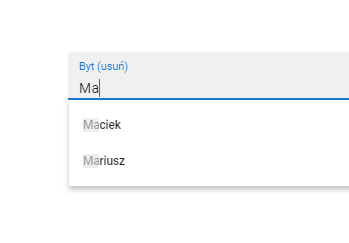
\includegraphics[width=.9\linewidth]{rys/nodes_autocompletion.png}}
      \caption{Autouzupełnianie}
    \end{subfigure}
    \caption{Wybór bytów do złączenia}
    \label{fig:input}
    \end{figure}
\newpage
\section{Link do repozytorium projektu}
    \url{https://github.com/Isild/ZIWG}
\end{document}